En oversigt over systemets arkitektur kan ses i figur \ref{fig:OverordnetArkitektur}. Systemet består af fire forskellige \textit{html}-sider. Forsiden er en login-side, hvor man enten kan logge ind på sin profil eller gå til en ny side, hvor man har mulighed for at oprette en profil. Når man har oprettet en profil, bliver man sendt tilbage til login-siden.
\newline
\noindent
Når man har logget ind, bliver man sendt til profil siden, hvor man kan oprette en ting til udlån og se en liste over ting. Herfra kan man gå til chat siden, hvor man har mulighed for at kommunikere med andre brugere.
\newline
\noindent
Til hver \textit{html}-side er der tilknyttet en \textit{css}-fil til at definere layoutet.


\begin{figure}[h]

\vspace{-20pt}
  \begin{center}
    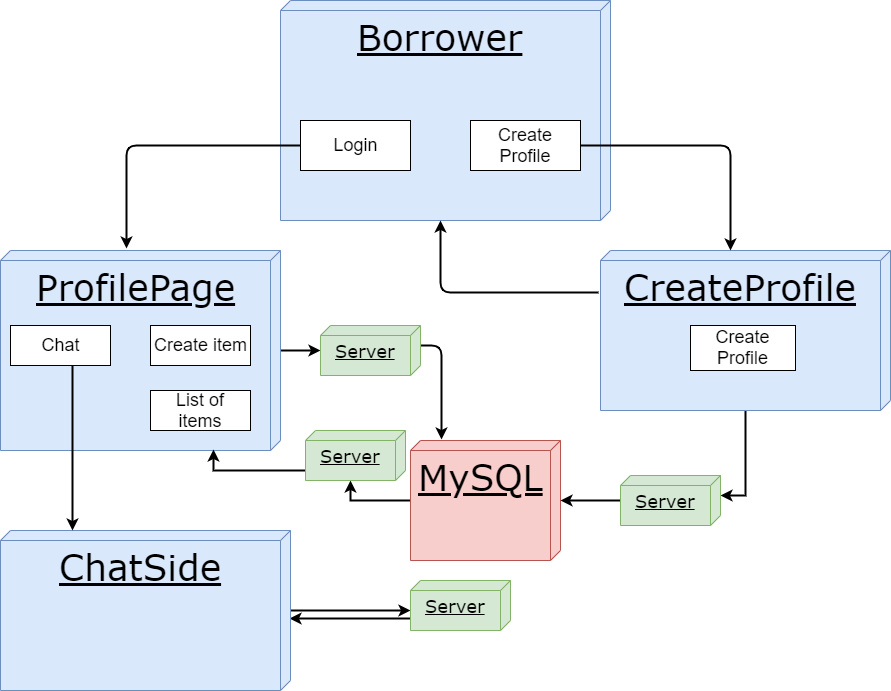
\includegraphics[scale=0.5]{Borrower.png}
    \caption{Diagram som viser hvordan systemets sider er forbundne.}
    \label{fig:OverordnetArkitektur}
  \end{center}
  \vspace{-10pt}
  \vspace{-20pt}
\end{figure} 
\noindent
Til at lagre informationer om brugeren, samt ting ejendele til udlån, har vi oprettet en \textit{MySql}-database. Databasen består af to tabeller: En \textit{users}-tabel og en \textit{items}-tabel. Figur ?? viser hvordan databasen er bygget op.
\newline
\noindent
Klient-siden af systemet er kodet i JavaScript, html og lagt ud i særskilte filer.
\newline
\noindent
Til at kommunikere med databasen har vi oprettet en webserver. Vi har valgt at bruge Node.js WebSocket-bibliotek, som er en to-vejs kommunikationsprotokol mellem \textit{server} og \textit{client}. WebSocket-bibliotek er en overbygning af HTTP-protokollen, og bliver initialiseret gennem et \textit{"handshake"} iværksat af klienten når den får forbindelse til serveren. Chattens funktionalitet er ligeledes bygget på Node.js WebSocket-bibliotek
